\documentclass[fontsize=14pt, paper=a4, pagesize, DIV=calc]{scrartcl}

\usepackage[T2A]{fontenc}
\usepackage[utf8]{inputenc}
\usepackage[russian]{babel}
\usepackage{color}
\usepackage{listings}
\usepackage{indentfirst} % Красная строка
\usepackage{setspace}
\usepackage{enumitem}
\usepackage{graphicx}
\usepackage{float}
\usepackage{paratype}

\setstretch{1.5}
\emergencystretch 5em

\lstset{
    basicstyle=\linespread{.94}\ttfamily,
    columns=fixed,
    breaklines=true,
    postbreak=\mbox{\textcolor{red}{$\hookrightarrow$}\space},
    belowskip=1ex,
    abovecaptionskip=0em,
    belowcaptionskip=1ex,
    aboveskip=1em,
    numbers=left,
    xleftmargin=1.5cm,
}

\renewcommand{\lstlistingname}{Листинг}
\renewcommand{\lstlistlistingname}{Список \lstlistingname ов}

\floatstyle{ruled}
\floatname{ListingEnv}{Листинг}
\newfloat{ListingEnv}{H}{lol}[section]

\def\code#1{\texttt{#1}}

\begin{document}

\begin{titlepage}

\centering

\vfill

МИНИСТЕРСТВО~ОБРАЗОВАНИЯ~И~НАУКИ~РФ

\vfill

Федеральное государственное автономное образовательное\\
учреждение высшего образования\\
ЮЖНЫЙ~ФЕДЕРАЛЬНЫЙ~УНИВЕРСИТЕТ

\vfill

Институт математики, механики и компьютерных наук\\
имени И.~И.~Воровича

\vfill

Направление подготовки\\
Фундаментальная информатика и информационные технологии

\vspace{2cm}

\textsf
{ИССЛЕДОВАНИЕ ДЕТАЛЕЙ РЕАЛИЗАЦИИ ОТЛАДЧИКА GHCI}

\vfill

Выпускная квалификационная работа

\vspace{2cm}

\raggedleft

Студента 4 курса\\
Д.~Ш.~Мирзоева

\vfill

Научный руководитель:\\
Старший преподаватель кафедры информатики и вычислительного эксперимента
Мехмата ЮФУ В.~Н.~Брагилевский

\vspace{2cm}

\raggedright

\noindent\begin{tabular}{ll}
\makebox[2.5in]{\hrulefill} & \makebox[2.5in]{\hrulefill}\\
оценка(рейтинг) & подпись руководителя\\
\end{tabular}

\vspace{2cm}

\centering

Ростов-на-Дону

2018

\end{titlepage}

\tableofcontents
\newpage

\section{Введение}

Отладка -- это процесс устранения ошибок в программе. Для его упрощения
разработчки используют специальные прогрммы-отладчики. Они обладают обширным
набором средств контроля за выполнением программы. 

Хотя все отладчики различаются с точки зрения функциональности, можно выявить
общие принципы работы, присущие большинству из них. К примеру, часто бывает
удобно остановить работу программы в месте предполагаемой ошибки и посмотреть
значения доступных в этот момент переменных. Кроме того, отладчики позволяют
выполнять программу ``шаг за шагом``, то есть выполнять каждый раз лишь одну
строку программы. Это помогает после остановки проследить изменение значений
переменных и саму последовательность выполнения инструкций.

В данной работе мы исследуем детали реализации отладчика языка Хаскель,
встроенного в интерпретатор GHCi. 

\subsection{Ленивость}

Особый интерес заключается в том, что Хаскель является языком программирования
с ленивой стратегией вычисления. Это означает, что порядок вычисления не задан
явно. Продемонстрируем эту особенность на двух примерах.

\begin{ListingEnv}
\caption{Делим два числа на Си}
\label{lst:divFooBarC}
\begin{lstlisting}[language=c]
int divFooBar(void) {
    int foo, bar;
    foo = ...;
    bar = ...;
    return foo / bar;
}
\end{lstlisting}
\end{ListingEnv}

В листинге \ref{lst:divFooBarC} приведён пример на языке Си. Последовательнось
выполнения \code{divFooBar} будет такой и только такой: сначала вычислится
значение \code{foo}, потом вычислится \code{bar}, потом вычислится результат.

\begin{ListingEnv}
\caption{Делим два числа на Хаскель}
\label{lst:divFooBarHaskell}
\begin{lstlisting}
divFooBar =
    let foo = ...
        bar = ...
    in foo `div` bar
\end{lstlisting}
\end{ListingEnv}

Код в листинге \ref{lst:divFooBarHaskell} делает то же самое. Разница
заключается в ленивости. Значения в Хаскель не вычисляются сразу. Вычисление
выражения начинается только в тот момент, когда понадобится его результат. В
связи с этим становится трудно сказать, в каком порядке будет выполняться
программа. \code{foo} и \code{bar} могут быть вычислены в любом порядке.

По этой причине GHCi имеет сложное устройство и не похож на отладчики
традиционных языков программирования.

\section{GHCi}

GHCi -- это интерпретатор Хаскель кода. Он является частью GHC, компилятора
языка Хаскель. GHCi позволяет вычислять значения и интерпритировать код. Кроме
того, в его состав входит отладчик.

\subsection{Команды отладчика}

\begin{itemize}
\item \code{:break} устанавливает точку останова;
\item \code{:force} и \code{:print} показывают значение выражения. Разница между ними в
том, что \code{:force} принудительно вычисляет его значение, а \code{:print} нет.
\item \code{:history} показывает последние выполненные шаги вычисления;
\item \code{:forward} и \code{:back} позволяют перемещаться по истории
вычислений вперед и назад соответственно;
\item \code{:trace} включает историю вычислений;
\item \code{:step} производит один шаг вычисления;
\item \code{:continue} продолжает выполнение вычисления после остановки.
\end{itemize}

\subsection{Пример работы с отладчиком GHCi}

Рассмотрим простую программу, осуществляющую сортировку списка целых чисел
алгоритмом бытрой сортировки.

\begin{ListingEnv}
\caption{main.hs}
\begin{lstlisting}
qsort [] = []
qsort (a:as) = qsort left ++ [a] ++ qsort right
 where 
  left  = filter (<=a) as
  right = filter (a<) as

main = print (qsort [8, 4, 0, 3, 1, 23, 11, 18])
\end{lstlisting}
\end{ListingEnv}

Загрузим её в интерпретатор.

\begin{ListingEnv}
\caption{}
\begin{lstlisting}[numbers=none]
$ ghci main.hs
Ok, modules loaded: Main.
*Main>
\end{lstlisting}
\end{ListingEnv}

Теперь можно добавить точку останова. Сделаем это на второй части определения
\code{qsort}.

\begin{ListingEnv}
\caption{}
\begin{lstlisting}[numbers=none]
*Main> :break 2
Breakpoint 0 activated at main.hs:2:16-47
\end{lstlisting}
\end{ListingEnv}

Команда \code{:break 2} устанавливает точку останова на строке 2 последнего
загруженного модуля. В нашем случае это \code{main.hs}. Она выбирает самое
левое полное подвыражение на этой строке(\code{qsort left ++ [a] ++ qsort
right}).

Теперь можно запустить программу.

\begin{ListingEnv}
\caption{}
\begin{lstlisting}[numbers=none]
*Main> :main
Stopped in Main.qsort, main.hs:2:16-47
_result :: [Integer] = _
a :: Integer = 8
left :: [Integer] = _
right :: [Integer] = _
[main.hs:2:16-47] *Main> 
\end{lstlisting}
\end{ListingEnv}

Выполнение приостановлено на точке останова. Подсказка ввода изменилась,
демонстрируя, что мы остановились и где мы остановились:
\code{main.hs:2:16-47}. Помимо этого выводится список доступных переменных.
Здесь можно заметить специальную переменную \code{\_result}, которая связана с
результатов текущего выражения. Для отображения значения переменной есть
команда \code{:print}.

\begin{ListingEnv}
\caption{}
\begin{lstlisting}[numbers=none]
[main.hs:2:16-47] *Main> :print left
left = (_t1::[Integer])
\end{lstlisting}
\end{ListingEnv}

Заметим, что \code{left} не был вычислен, поэтому в его отображении отсутствует
полный список значений. Можно потребовать его вычисления. Для этого существует
команда \code{:force}. 

\begin{ListingEnv}
\caption{}
\begin{lstlisting}[numbers=none]
[main.hs:2:16-47] *Main> :force left
left = [4,0,3,1]
\end{lstlisting}
\end{ListingEnv}

Стоит отметить, что вычисление подвыражения может не завершаться или
завершаться с ошибкой даже в том случае, когда вычисление выражение целиком
завершается успешно. Рассмотрим пример.

\begin{ListingEnv}
\caption{main.hs}
\begin{lstlisting}
a = 0
b = 1 `div` a
foo = if a == 0 then 0 else b
\end{lstlisting}
\end{ListingEnv}

Результатом вычисления foo будет ноль, а вовсе не ошибка, как можно подумать,
заметив деление на ноль в строке 2. Это происходит благодаря ленивой стратегии
вычисления. Значение \code{b} не вычисляется, потому что его результат не
требуется для вычисления \code{foo}.

\subsection{История вычислений}

В традиционных отладчиках существует понятие стека вызова функций. После
остановки в некотором месте программы он помогает понять, откуда мы туда
пришли. 

Стек состоит из адресов возврата функций, которые вычисляются в данный момент,
в порядке обратном порядку их вызова. По нему можно перемещаться, выясняя
значения локальных переменных в этих функциях.

Похожий доступ к стеку можно получить и в Хаскель, но это требует компиляции с
опцией \code{-prof}, которая включает оснащение кода системой профилирования.
Такой режим компиляции несовместим с отладчиком. 

Существует альтернатива --- история вычислений. Выражения в Хаскель вычисляются
по мере необходимости, поэтому важнее стека вызовов может оказаться именно
последовательность предпринятых шагов вычисления. Историю таких шагов можно
получить с помощью команд \code{:trace} и \code{:hist}. Рассмотрим пример.

\begin{ListingEnv}
\caption{}
\begin{lstlisting}[numbers=none]
*Main> :list qsort
1  qsort [] = []
2  qsort (a:as) = qsort left ++ [a] ++ qsort right
*Main> :b 1
Breakpoint 0 activated at main.hs:1:12-13
\end{lstlisting}
\end{ListingEnv}

Запустим сортировку небольшого списка с трассировкой с помощью команды \code{:trace}.

\begin{ListingEnv}
\caption{}
\begin{lstlisting}[numbers=none]
*Main> :trace qsort [3, 2, 1]
Stopped in Main.qsort, main.hs:1:12-13
_result :: [a] = _
\end{lstlisting}
\end{ListingEnv}

Теперь мы можем посмотреть историю шагов вычисления. Для этого есть команда
\code{:hist}.

\begin{ListingEnv}
\caption{}
\begin{lstlisting}[numbers=none]
[main.hs:1:12-13] *Main> :hist
-1  : qsort:left (main.hs:4:12-26)
-2  : qsort (main.hs:2:16-25)
-3  : qsort (main.hs:2:16-47)
-4  : qsort:left (main.hs:4:12-26)
-5  : qsort (main.hs:2:16-25)
-6  : qsort (main.hs:2:16-47)
-7  : qsort:left (main.hs:4:12-26)
-8  : qsort (main.hs:2:16-25)
-9  : qsort (main.hs:2:16-47)
<end of history> 
\end{lstlisting}
\end{ListingEnv}

Для перемещения по истории используются команды \code{:forward} и
\code{:backward}. Следом удобно использовать команду \code{:list}, которая
отображает исходный код места, на котором мы остановились и выделяет 
вычисляемое выражение.

\begin{ListingEnv}
\caption{}
\begin{lstlisting}[numbers=none]
[main.hs:1:12-13] *Main> :back
Logged breakpoint at main.hs:4:12-26
_result :: [Integer]
a :: Integer
as :: [Integer]
[-1: main.hs:4:12-26] *Main> :list
3   where
4     left  = >>> filter (<=a) as <<<
5     right = filter (a<) as
[-1: main.hs:4:12-26] *Main> :forward
Stopped at main.hs:1:12-13
_result :: [a]
[main.hs:1:12-13] *Main> :list
1  qsort [] = >>> [] <<<
2  qsort (a:as) = qsort left ++ [a] ++ qsort right
\end{lstlisting}
\end{ListingEnv}

\section{Компиляция}

\begin{figure}[H]
\centering
\caption{Схема процесса компиляции}
\label{fig:compilation}
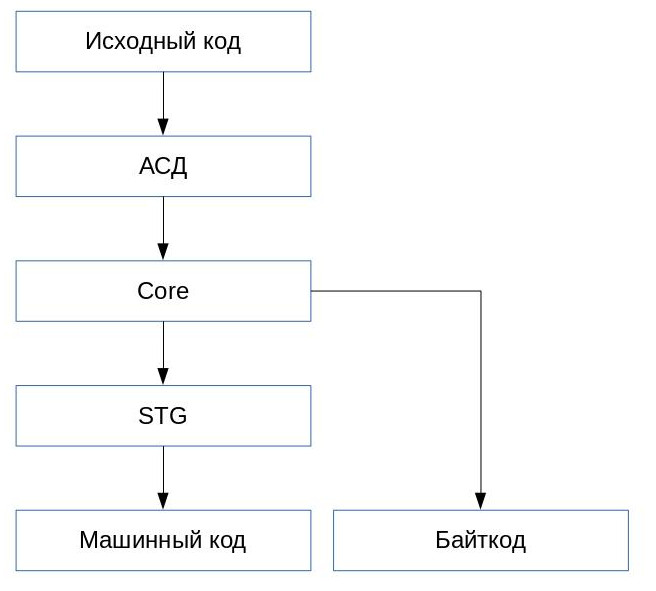
\includegraphics[scale=0.8]{compilation.jpg}
\end{figure}

На рисунке \ref{fig:compilation} приведена схема процесса компиляции.
Рассмотрим её более подробно. В прямоугольниках обозначена форма представления
программы на текущем этапе.

\subsection{Машинный код}

При компиляции отдельного файла на выходе получается исполняемый или объектный
файл, то есть машинный код. 

На вход компилятору поступает файл с исходным кодом. Он рассматривается как 
последовательность символов.

Эту последовательность символов обрабатывает лексический анализатор Alex и
превращает её в последовательность лексем. Последовательность лексем
обрабатывает синтаксический анализатор Happy и превращает её в абстрактное
синтаксическое дерево. Делее происходит проверка типов.

Следующий этап --- удаление синтаксического сахара. Хаскель транслируется в
промежуточный язык Core. Он имеет гораздо более простой синтаксис. На этом шаге
происходят многочисленные оптимизации. Использование компактного промежуточного
языка позволяет упростить код связанный с оптимизацией и сделать его в
некоторой мере независимым от синтаксиса самого языка.

Последний шаг --- кодогенерация. Прежде всего Core транслируется в язык STG.
STG код транслируется в C-{}-. Это низкоуровневый императивный язык, который
используется в качестве переносимого ассемблера. Он может быть скомпилирован
напрямую в машинный код, а может быть транслирован в ещё одно промежуточное
представление: llvm или C. Это обеспечивает более высокий уровень оптимизации.

\subsubsection{Немного об STG}

STG это абстрактная машина для свёртки графов(Simon L Peyton Jones
\cite{funcOnStockHard}). Она была разработана специально для компиляции
функциональных языков в низкоуровневое машинное представление.  STG язык -- это
язык команд этой машины. Он оперирует понятиями, которые легко отобразить на
существующие процессоры. Среди них стек, куча, регистры. 

STG расшифровывается как Spineless Tagless G-machine.

\begin{itemize}

\item \textbf{Spineless} означает, что у этой машины отсутствует spine. Spine -- это стек
укзазателей на самые левые узлы дерева.

\begin{figure}[H]
\centering
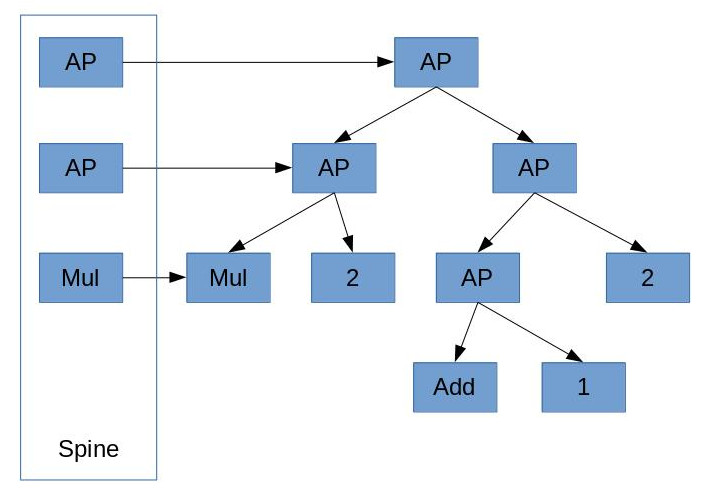
\includegraphics[scale=0.7]{spine.jpg}
\end{figure}

\item Структура объектов, которыми оперирует STG, похожа. Все они имеют первым
полем указатель на код, который нужно выполнить, чтобы вычислить их значение.
Поэтому для не нужно знать точный тип вычисляемого объекта. 

В структуре объектов отсутствует поле, обозначающее тип, то есть tag. Отсюда
\textbf{tagless} в
названии.

\item \textbf{G-machine} это сокращение от Graph reduction machine, то есть
машина графовых свёрток. Здесь граф --- это выражение на функциональном языке, а
свёртка --- это процесс его вычисления.

\end{itemize}

\subsection{Байткод}

Интерпретатор использует другой выходной формат. На выходе от компилятора он
требует Byte Code Object(BCO). В отличие от стандартной кодогенерации, входом
которой служит код С-{}-, входом генератора байткода служит Core.

\begin{ListingEnv}
\caption{compiler/llvm/LlvmCodeGen.hs}
\begin{lstlisting}[firstnumber=44]
llvmCodeGen :: DynFlags -> Handle -> UniqSupply
               -> Stream.Stream IO RawCmmGroup ()
               -> IO ()
\end{lstlisting}
\end{ListingEnv}

\begin{ListingEnv}
\caption{compiler/nativeGen/AsmCodeGen.hs}
\begin{lstlisting}[firstnumber=108]
nativeCodeGen :: DynFlags -> Module -> ModLocation -> Handle -> UniqSupply
              -> Stream IO RawCmmGroup ()
              -> IO UniqSupply
\end{lstlisting}
\end{ListingEnv}

\begin{ListingEnv}
\caption{compiler/ghci/ByteCodeGen.hs}
\begin{lstlisting}[firstnumber=81]
byteCodeGen :: HscEnv
            -> Module
            -> CoreProgram
            -> [TyCon]
            -> Maybe ModBreaks
            -> IO CompiledByteCode
\end{lstlisting}
\end{ListingEnv}

\code{BCO} -- это один из объектов, которыми оперирует STG. Он представлет из
себя массив инструкций байткода. Интерпретацией этих объектов занимется среда
времени выполнения. Интерпретатор во время своей работы взяимодействует со
средой времени выполнения, для исполнения своих команд.

\begin{ListingEnv}
\caption{rts/Interpreter.c}
\begin{lstlisting}[firstnumber=295]
Capability *
interpretBCO (Capability* cap)
{
\end{lstlisting}
\end{ListingEnv}

\section{Баг}

В рамках исследования реализации отладчика мы обратили внимание на баг(\#{}8316,
\cite{bug}). Он заключается в том, что отладчик аварийно завершается при попытке
вычислить определённую переменную после остановки.

\subsection{Воспроизведение}

Для демонстрации ошибки рассмотрим файл Test.hs:

\begin{ListingEnv}
\caption{Test.hs}
\begin{lstlisting}
foo :: [Int]
foo = [1..]
\end{lstlisting}
\end{ListingEnv}

Загрузим его в интерпретатор

\begin{ListingEnv}
\caption{}
\begin{lstlisting}[numbers=none]
ghci Test.hs
\end{lstlisting}
\end{ListingEnv}

Поставим точку останова на \code{foo}, запустим его вычисление и
напечатаем с помощью команды \code{:print}.

\begin{ListingEnv}
\caption{}
\begin{lstlisting}[numbers=none]
*Main> :break foo
Breakpoint 0 activated at main.hs:2:7-11
*Main> foo
Stopped in Main.foo, main.hs:2:7-11
_result :: [Int] = _
[main.hs:2:7-11] *Main> :print foo
foo = (_t1::[Int])
\end{lstlisting}
\end{ListingEnv}

Теперь попробуем вычислить значение \code{\_t1}.

\begin{ListingEnv}
\caption{}
\begin{lstlisting}[numbers=none]
[main.hs:2:7-11] *Main> _t1
\end{lstlisting}
\end{ListingEnv}

Здесь возникает ошибка и интерпретатор аварийно завершается.

\begin{ListingEnv}
\caption{Ошибка}
\begin{lstlisting}[numbers=none]
<interactive>: internal error: TSO object entered!
    (GHC version 8.5.20180302 for x86_64_unknown_linux)
    Please report this as a GHC bug:  http://www.haskell.org/ghc/reportabug
[1]    5445 abort (core dumped)  ghci Test.hs
\end{lstlisting}
\end{ListingEnv}

\section{Архитектура отладчика GHCi}

Основные локации:

\begin{itemize}

\item \textbf{\texttt{ghc/GHCi}}

В папке ghc/GHCi находится код реализующий взаимодействие с пользователем:
распознавание и выполнение функций соответствующих команд.

\item \textbf{\texttt{libraries/ghci}}

Содержит:

\begin{itemize}
\item Типы для межпроцессной обработки значений
\item Протокол взаимодействия
\item Реализацию сообщений
\item Реализацию расширения Template Haskell для отладчика
\end{itemize}

\item \textbf{\texttt{iserv}}

Процесс-сервер отладчика. Код довольно простой. Большая часть реализации
содержится в libraries/ghci

\item \textbf{\texttt{compiler/ghci}}

Модуль compiler/ghci предоставляет интерфейс сервера, который используется
остальным кодом.

\item \textbf{\texttt{rts/Interpreter.c}}

Содержит код системы времени выполнения, отвечающий за исполнение байткода. 
Функция \texttt{interpretBCO}.

\item \textbf{\texttt{include/rts/Bytecodes.h}}

Содежит номера байткод инструкций.

\begin{ListingEnv}
\caption{include/rts/Bytecodes.h}
\begin{lstlisting}[firstnumber=26]
#define bci_STKCHECK            1
#define bci_PUSH_L              2
#define bci_PUSH_LL             3
#define bci_PUSH_LLL            4
#define bci_PUSH8                       5
#define bci_PUSH16                      6
...
\end{lstlisting}
\end{ListingEnv}

\end{itemize}

\subsection{Выполнение}

Рассмотрим что происходит, когда мы запускаем интерпретатор. Во первых отметим,
что ghci не является отдельной от компилятора утилитой. Это скрипт, который
запускает компилятор, то есть ghc, с параметром -{}-interactive.

\begin{ListingEnv}
\caption{}
\begin{lstlisting}[numbers=none]
user@desktop:~$ which ghci
/usr/bin/ghci
user@desktop:~$ cat /usr/bin/ghci
#!/bin/sh
exec "/usr/bin/ghc-8.0.1" --interactive "$@"
\end{lstlisting}
\end{ListingEnv}

Теперь обратимся к коду. Функция \code{main}, с которой начинается выполнение
ghc, находится в файле ghc/Main.hs. Там происходит анализ параметров командной
строки. Если среди параметров есть \code{-{}-interactive}, то вызывается
функция \code{interactiveUI}. 

Главной монадой в ghc является монада Ghc. Она позволяет осуществлять
ввод-вывод и обеспечивает доступ к состоянию компилятора: флаги настроек, граф
модулей и другие. 

\begin{ListingEnv}
\caption{compiler/main/GhcMonad.hs}
\begin{lstlisting}[numbers=none]
newtype Ghc a = Ghc { unGhc :: Session -> IO a }
\end{lstlisting}
\end{ListingEnv}

Модули компилятора, которые требуют больше возможностей расширяют эту монаду.
Интерпретатор пользуется монадой GHCi. Она помимо возможностей монады Ghc
обеспечивает доступ к состоянию интерпретатора: загруженные модули, подсказка
ввода, количество введённых строк и другие.

\begin{ListingEnv}
\caption{ghc/UI/Monad.hs}
\begin{lstlisting}[numbers=none]
newtype GHCi a 
    = GHCi { unGHCi :: IORef GHCiState -> Ghc a }
\end{lstlisting}
\end{ListingEnv}

\code{interactiveUI} настраевает стандартные буферы для интерактивной работы и
запускает \code{runGHCi}. Её результат передаётся аргументом для
\code{startGHCi}, потому что значение результата имеет тип \code{GHCi ()}, а
\code{interactiveUI} возвращает тип \code{Ghc ()}.

\begin{ListingEnv}
\caption{ghc/GHCi/UI.hs}
\begin{lstlisting}[firstnumber=400]
interactiveUI 
  :: GhciSettings 
  -> [(FilePath, Maybe Phase)] 
  -> Maybe [String]
  -> Ghc ()
interactiveUI config srcs maybe_exprs = do
\end{lstlisting}
...
\begin{lstlisting}[firstnumber=454]
    startGHCi (runGHCi srcs maybe_exprs)
        GHCiState{ progname = default_progname,
                   args     = default_args, ... }
\end{lstlisting}
\end{ListingEnv}

Для взаимодействия с пользователем ghc использует библиотеку haskeline. Она
похожа на библиотеку realine для си. Ввод строк происходит в монаде InputT.
\code{runGHCi} запускает read-eval-print loop, который работает в этой монаде.

\begin{ListingEnv}
\caption{ghc/GHCi/UI.hs}
\begin{lstlisting}[firstnumber=892]
-- | The main read-eval-print loop
runCommands :: InputT GHCi (Maybe String) -> InputT GHCi ()
runCommands gCmd = runCommands' handler Nothing gCmd >> return ()
\end{lstlisting}
\end{ListingEnv}

\code{runCommands'} вызывает \code{runOneCommand}, которая вызвыает
\code{doCommand}. Если ввод начинается с двоеточия \code{doCommand} распознаёт
команду и запускает её обработчик. В противном случае считается, что
пользователь ввёл выражение.

\paragraph{Команда}

Если введённая строка начинается с восклицательного знака, то в этом случае её
остальная часть рассматривается как команда шел скрипта.

\begin{ListingEnv}
\caption{ghc/GHCi/UI.hs}
\begin{lstlisting}[firstnumber=1204]
specialCommand :: String -> InputT GHCi Bool
specialCommand ('!':str) = lift $ shellEscape (dropWhile isSpace str)
\end{lstlisting}
...
\begin{lstlisting}[firstnumber=1221]
shellEscape :: String -> GHCi Bool
shellEscape str = liftIO (system str >> return False)
\end{lstlisting}
\end{ListingEnv}

Если строка не начинается с восклицательного знака, то из неё выделяется первое
слово. По нему происходит поиск в списке команд и макросов. 

\begin{ListingEnv}
\caption{ghc/GHCi/UI.hs}
\begin{lstlisting}[firstnumber=1206]
specialCommand str = do
  let (cmd,rest) = break isSpace str
  maybe_cmd <- lift $ lookupCommand cmd

  case maybe_cmd of
    GotCommand cmd -> (cmdAction cmd) (dropWhile isSpace rest)
\end{lstlisting}
\end{ListingEnv}

Активные макросы и команды доступны в монаде \code{GHCi}. Список макросов
изначально пуст. Пользователь может определить свои макросы с помощью команды
\code{:def}. Список команд доступных в интерпретаторе по умолчанию находится в
переменной \code{ghciCommands}, которая определена в этом же файле. В этом
списке помимо названий команд находятся соответсвующие им функции.

\paragraph{Код}

Если пользователь ввёл код, работает функция \code{runStmt}.

\begin{ListingEnv}
\caption{ghc/GHCi/UI.hs}
\begin{lstlisting}[firstnumber=1080]
runStmt :: String -> SingleStep -> GHCi (Maybe GHC.ExecResult)
runStmt stmt step = do
  dflags <- GHC.getInteractiveDynFlags
  if | GHC.isStmt dflags stmt    -> run_stmt
     | GHC.isImport dflags stmt  -> run_import
     | otherwise                 -> run_decl
\end{lstlisting}
\end{ListingEnv}

Код бывает трёх видов: это может быть просьба загрузить модуль(\code{import}),
объявление переменной или функции(\code{declaration}),
выражение(\code{statement}).

Рассмотрим подробно случаи объявления и выражения.

\paragraph{Объявление}

В случае объявления работа продолжается в монаде \code{GHC}. Вызывается функция
\code{runDeclsWithLocation}.

\begin{ListingEnv}
\caption{compiler/main/InteractiveEval.hs}
\begin{lstlisting}[firstnumber=199]
runDeclsWithLocation :: GhcMonad m => String -> Int -> String -> m [Name]
runDeclsWithLocation source linenumber expr =
...
    (tyThings, ic) <- liftIO $ hscDeclsWithLocation hsc_env expr source linenumber
...
\end{lstlisting}
\end{ListingEnv}

\code{hscDeclsWithLocation} выполняет все стадии компиляции: лексический и
синтаксический анализ, разрешение имён, проверка типов, удаление
синтаксического сахара, оптимизация и кодогенерация, а также линковка.  Она
возвращает новый интактивный контекст и новые доступные идентификаторы:
функции, переменные, геттеры структур, методы классов.

\paragraph{Выражение}

В случае выражения работает функция \code{execStmt}. Она сначала компилирует, а
затем выполняет введёный пользователем код.

\begin{ListingEnv}
\caption{compiler/main/InteractiveEval.hs}
\begin{lstlisting}
-- | Run a statement in the current 
     interactive context.
execStmt
  :: GhcMonad m
  => String -- ^ a statement (bind or expression)
  -> ExecOptions
  -> m ExecResult
execStmt stmt ExecOptions{..} = do
...
    -- compile to value (IO [HValue]), don't run
    r <- liftIO $ 
        hscStmtWithLocation hsc_env' stmt 
                            execSourceFile 
                            execLineNumber
...
    evalStmt hsc_env' (isStep execSingleStep) (execWrap hval)
\end{lstlisting}
\end{ListingEnv}

В конце концов управление переходит в функцию \code{sandboxIO}.

\begin{ListingEnv}
\caption{libraries/ghci/GHCi/Run.hs}
\begin{lstlisting}[numbers=none]
sandboxIO :: EvalOpts -> IO a -> IO (EvalStatus a)
sandboxIO opts io = do
  -- We are running in uninterruptibleMask
  breakMVar <- newEmptyMVar
  statusMVar <- newEmptyMVar
  withBreakAction opts breakMVar statusMVar $ do
    measureAlloc $ tryEval $ rethrow opts 
                 $ clearCCS io
\end{lstlisting}
\end{ListingEnv}

\code{MVar} это изменяемая переменная, одной из функций которой служит
синхронизация потоков. Она может находиться в двух состояниях: пустая или
хранит значение. При помещении в неё значения, если она не пустая, поток будет
заблокирован, пока какой-нибудь другой поток не опустошит её. Также блокировка
происходит при изъятии, если в переменной нет значения.

\code{sandboxIO} создаёт новый поток, запускает в нём введённый код и начинает
ждать, когда в переменной \code{statusMVar} появится статус выполнения. Статус
это либо завершение, либо остановка на точке останова. 

В момент, когда затрагивается точка останова, поток, выполняющий код
пользователя, заполняет изменяемую переменную \code{statusMVar} значением
\code{EvalBreak} и пытается достать значение из переменной \code{breakMVar}.
Первое позволяет разблокировать поток \code{ghci}, второе даёт возможность
потоку \code{ghci} продолжить выполнения с места остановки.

\subsection{RTS}

Во время удаления синтаксического сахара в АСД внедряются специальные узлы
\code{HsTick}. Это необходимо для установки соответствия между кодом на
последующих этапах и исходным кодом программы. Они используются для проверки
покрытия кода тестами и в отладчике для реализации точек остановки. Все
выражения, подвыражения и сами объявления оборачиваются в этот конструктор.

При компиляции \code{HsTick} добавляется специальная инструкция байткода
\code{BRK\_FUN}. Код интерпретации данной инструкции находится в файле
\code{rts/Interpreter.c} в функции \code{interpretBCO}. Когда выполнение
доходит до этой инструкции, происходит следующее. Интерпретатор проверяет
активна ли точка останова соответствующая этой инструкции. Информация об этом
хранится в специальном массиве бит внутри \code{BCO}. У инструкции
\code{BRK\_FUN} есть параметр -- индекс в этом массиве. Установка
соответствующего бита активирует точку останова.  Если точка неактивна, то
выполнение продолжается.  В противном случае выполняется код, который
использует изменяемые переменные из \code{sandboxIO}.

\addcontentsline{toc}{subsection}{Библиография}
\begin{thebibliography}{9}

\bibitem{funcOnStockHard}
Simon L Peyton Jones,
\emph{Implementing lazy functional languages on stock hardware: the Spineless
Tagless G-machine}, 1992

\bibitem{bug}
GHCi debugger segfaults when trying force a certain variable
\emph{https://ghc.haskell.org/trac/ghc/ticket/8316}

\end{thebibliography}

\end{document}
